\documentclass{TDP003mall}
\usepackage{graphicx}
\graphicspath{ {bilder/} }



\newcommand{\version}{Version 1.0}
\author{Pia Løtvedt, \url{pialo059@student.liu.se}\\
  Isabella Delgado, \url{isade842@student.liu.se}\\
  Sabrina Bjurman, \url{sebbj070@student.liu.se}}
\title{LoFi-prototyp}
\date{2017-09-12}
\rhead{Pia Løtvedt\\
Isabella Delgado\\
Sabrina Bjurman}

\begin{document}
\projectpage

\tableofcontents

\pagebreak
\section{LoFi-prototypens syfte}

En LoFi-prototyp ska representera en modell av det slutliga systemet. Tanken är att det ska gå relativt fort att ta fram en LoFi-prototyp, men den ska samtidigt vara välgenomtänkt. Prototypen kan därefter användas för att testa layout och användargränssnitt och planera arbetet med att implementera systemet.


\pagebreak
\section{Portfolions struktur}

LoFi-prototypen visar layout och gränssnitt för fyra webbsidor som ska finnas med i projektet. Dessa sidor är framsida, en sida med lista över projekt och sökmöjligheter, en sida med lista
over tekniker och möjlighet att visa projekt med där tekniken ingår, samt en sida med information om ett specifikt projekt.

\subsection{Meny}

Menyn, se. Figur~\ref{fig1:Framsida} finns tillgänglig på alla sidor i portfolion och innehåller flera länkar som navigerar till olika sidor. De olika navigeringspunkterna i menyn är ''Home'', ''Projects'' och ''Techniques''. Samtliga navigationspunkter tar användaren till andra sidor i portfolion. De specifika sidorna tas upp senare i dokumentet. När användaren befinner sig på en viss sida är navigeringspunkten för den aktuella sidan understruken.

Under menyn, se t.ex. Figur~\ref{fig1:Framsida} finns det en streckad linje som visar att sektionen ovan följer med när man scrollar ner på sidorna. Den streckade linjen är ingenting användaren ser på portfolion, detta är endast ett navigationsförtydligande för LoFi-prototypen.


\pagebreak
\subsection{Framsida}

\begin{figure}[ht!]
  \centering
  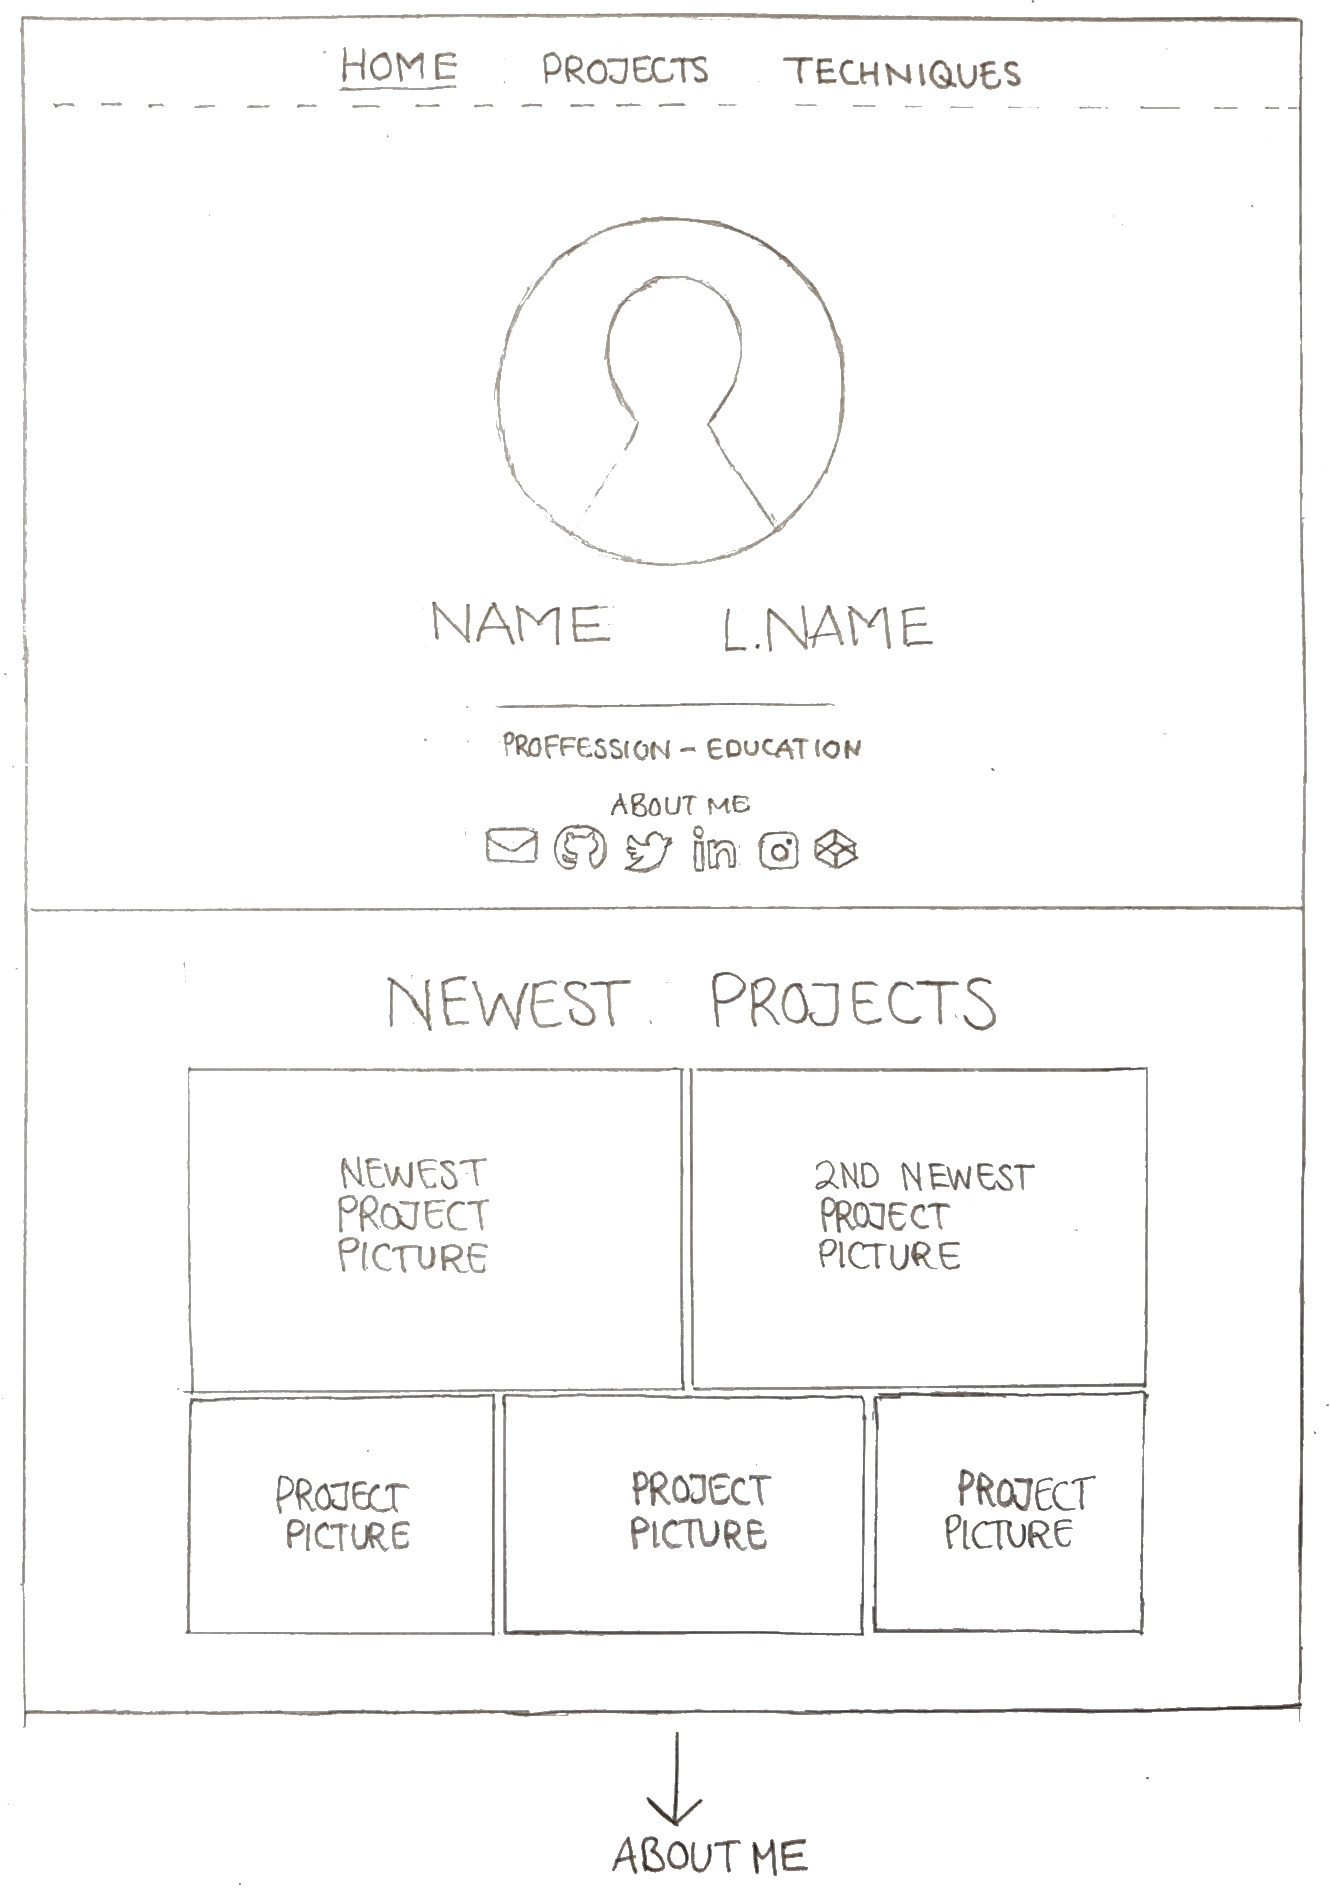
\includegraphics[width=140mm]{1_home.jpg}
  \caption{Framsida för portfolio.} \label{fig1:Framsida}
\end{figure}

På framsidan finns det ett porträtt på ägaren av portfolion som man kan trycka på för att ta sig vidare ner på framsidan till ''About Me'' sektionen, se Figur~\ref{fig2:AboutMe}. Det går även att trycka på länken som heter ''About Me'' för att komma dit.

Under länken ''About Me'' finns det symboler som tar dig till ägarens sidor på olika sociala medier samt en symbol för e-post. När man trycker på symbolen för e-post kommer det visas en flytande ruta med ägarens e-post adress som man kan kopiera. Detta finns både under ägarens porträtt samt sektionen ''About Me'' som ses på Figur~\ref{fig2:AboutMe}. På sektionen ''About Me'' finns det även en ikon som visar en pil. Det går att trycka på ikonen för att ta sig till toppen av sidan.

Nedanför porträttet finns det en sektion som heter ''Newest Projects''. Där visas de senaste projekten i ordningen ''Newest project'', ''2nd newest project'' samt övriga projekt. Dessa representeras som bilder som går att hålla över för att se en kort beskrivning av ett projekt. Trycker man på bilden tas man till det enskilda projektets sida, detta förklaras mer under rubrik~\ref{EnskildaProjekt}.

\begin{figure}[h]
  \centering
  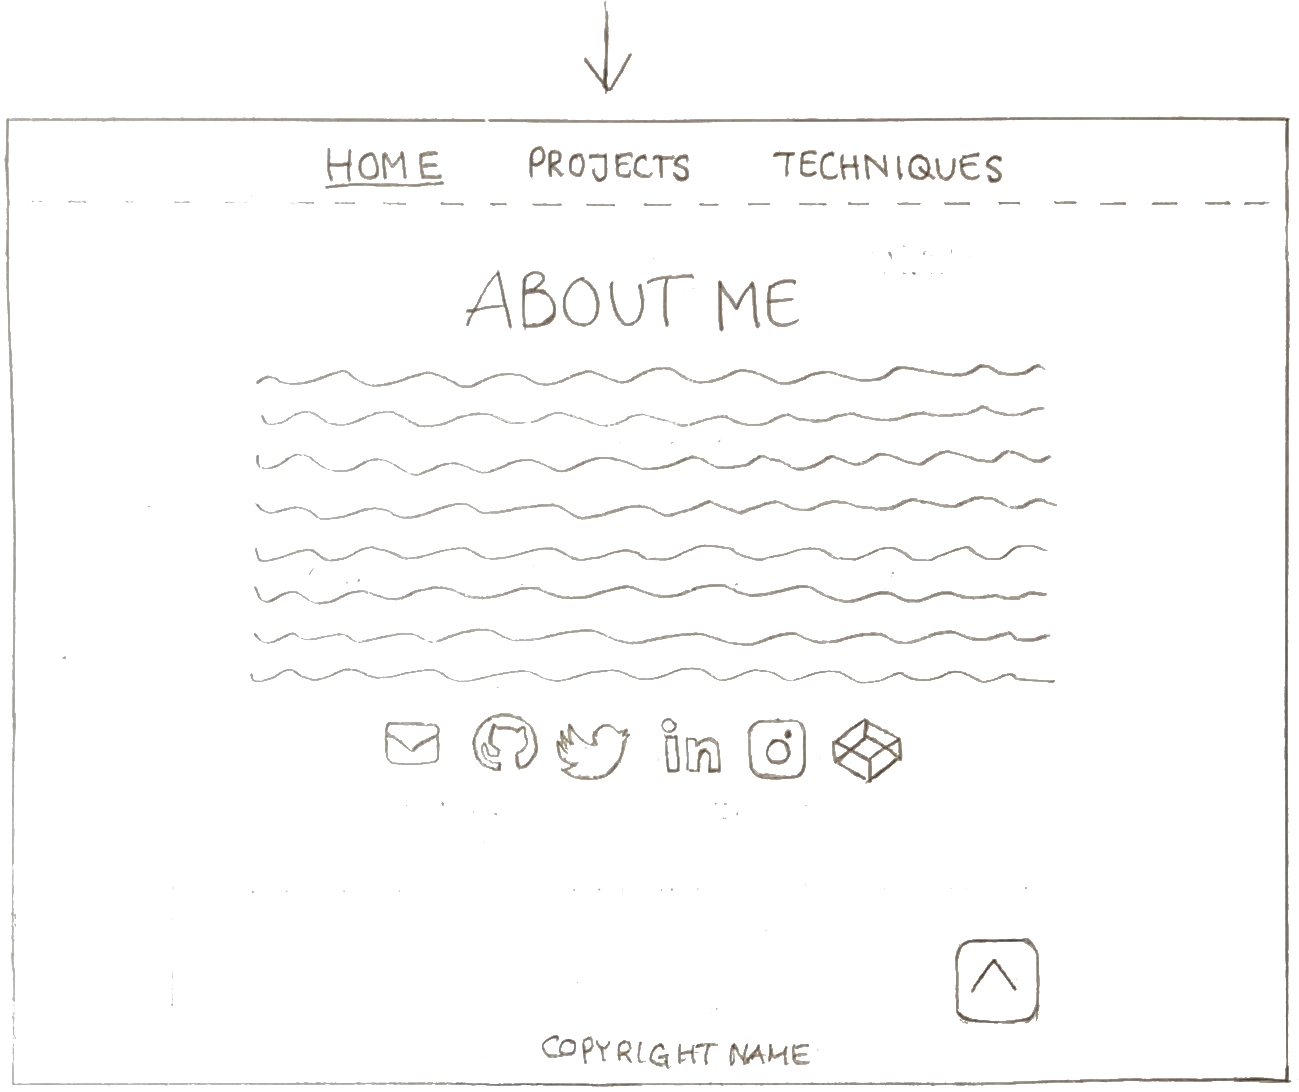
\includegraphics[width=140mm]{2_aboutme.jpg}
  \caption{Sektion på framsida, ''About Me''.} \label{fig2:AboutMe}
\end{figure}




\pagebreak
\subsection{Projektlista}

\begin{figure}[ht!]
  \centering
  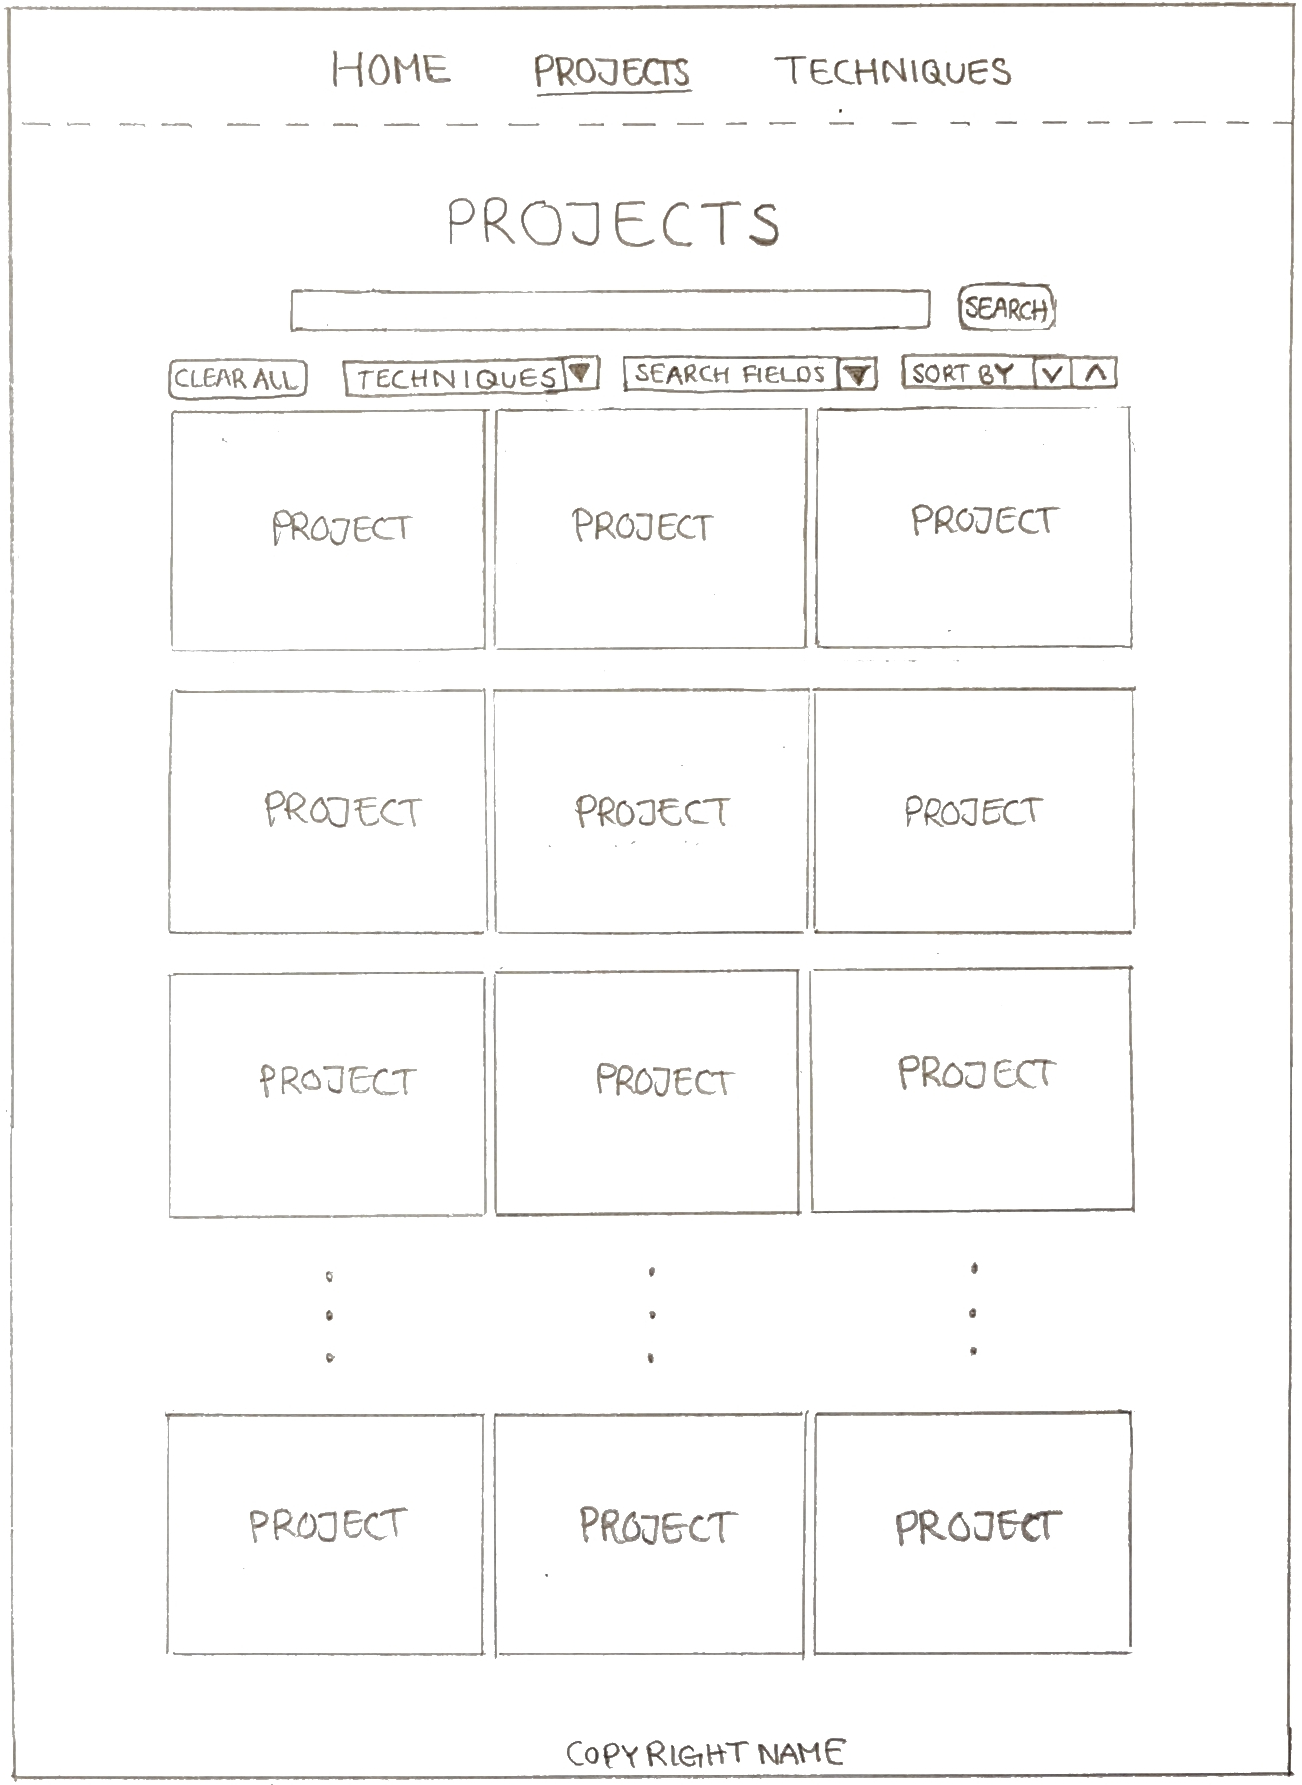
\includegraphics[width=140mm]{3_projects.jpg}
  \caption{Projektsidan, lista med projekt som visas på sidan.} \label{fig3:Projects}
\end{figure}


\pagebreak
Sidan ska visa en lista över alla projekt som finns i portfolion. Längst upp finns en navigeringsbar som följer med sidan när användaren scrollar ner. Under rubriken ''Projects'' finns en sökbar för att låta användaren söka bland projekten. Bredvid sökbaren finns en knapp som användaren kan trycka på för att söka. I anslutning till sökbaren finns knappen ''Clear All'' som rensar sökfält och filter, en drop-down meny där användaren kan sortera projekten på specifika tekniker, en till drop-down meny där användaren kan välja ett eller flera sökfält och en tredje drop-down meny där användaren kan välja vilket fält resultaten ska sorteras på. Bredvid sistnämnda sökfält finns två knappar med pil ner och pil upp, där användaren kan bestämma om sorteringen ska göras i fallande eller stigande ordning.

Vid sökning skriver användaren in valfri text i sökbaren samt väljer eventuella filter och sökfält.
Om användaren ändrar tekniker eller sortering ska sökresultatet uppdateras direkt. Om sökfält ändras så ska sökresultatet endast uppdateras vid en ny sökning.

Drop-down menyn för tekniker kommer att innehålla en lista med de tekniker som har använts i minst ett projekt.

I drop-down menyn för sökfält ''Search Fields'' kommer följande alternativ att finnas:
\begin{itemize}
  \item Projektnamn
  \item Årtal
  \item Kurskod
  \item Kursnamn
  \item Kurspoäng
\end{itemize}

I sorteringsmenyn ''Sort By'' ska det vara möjligt att välja att sortera (stigande eller fallande) efter följande:
\begin{itemize}
  \item Projektnamn
  \item Datum
\end{itemize}


\pagebreak
\subsection{Tekniksida}

\begin{figure}[h]
  \centering
  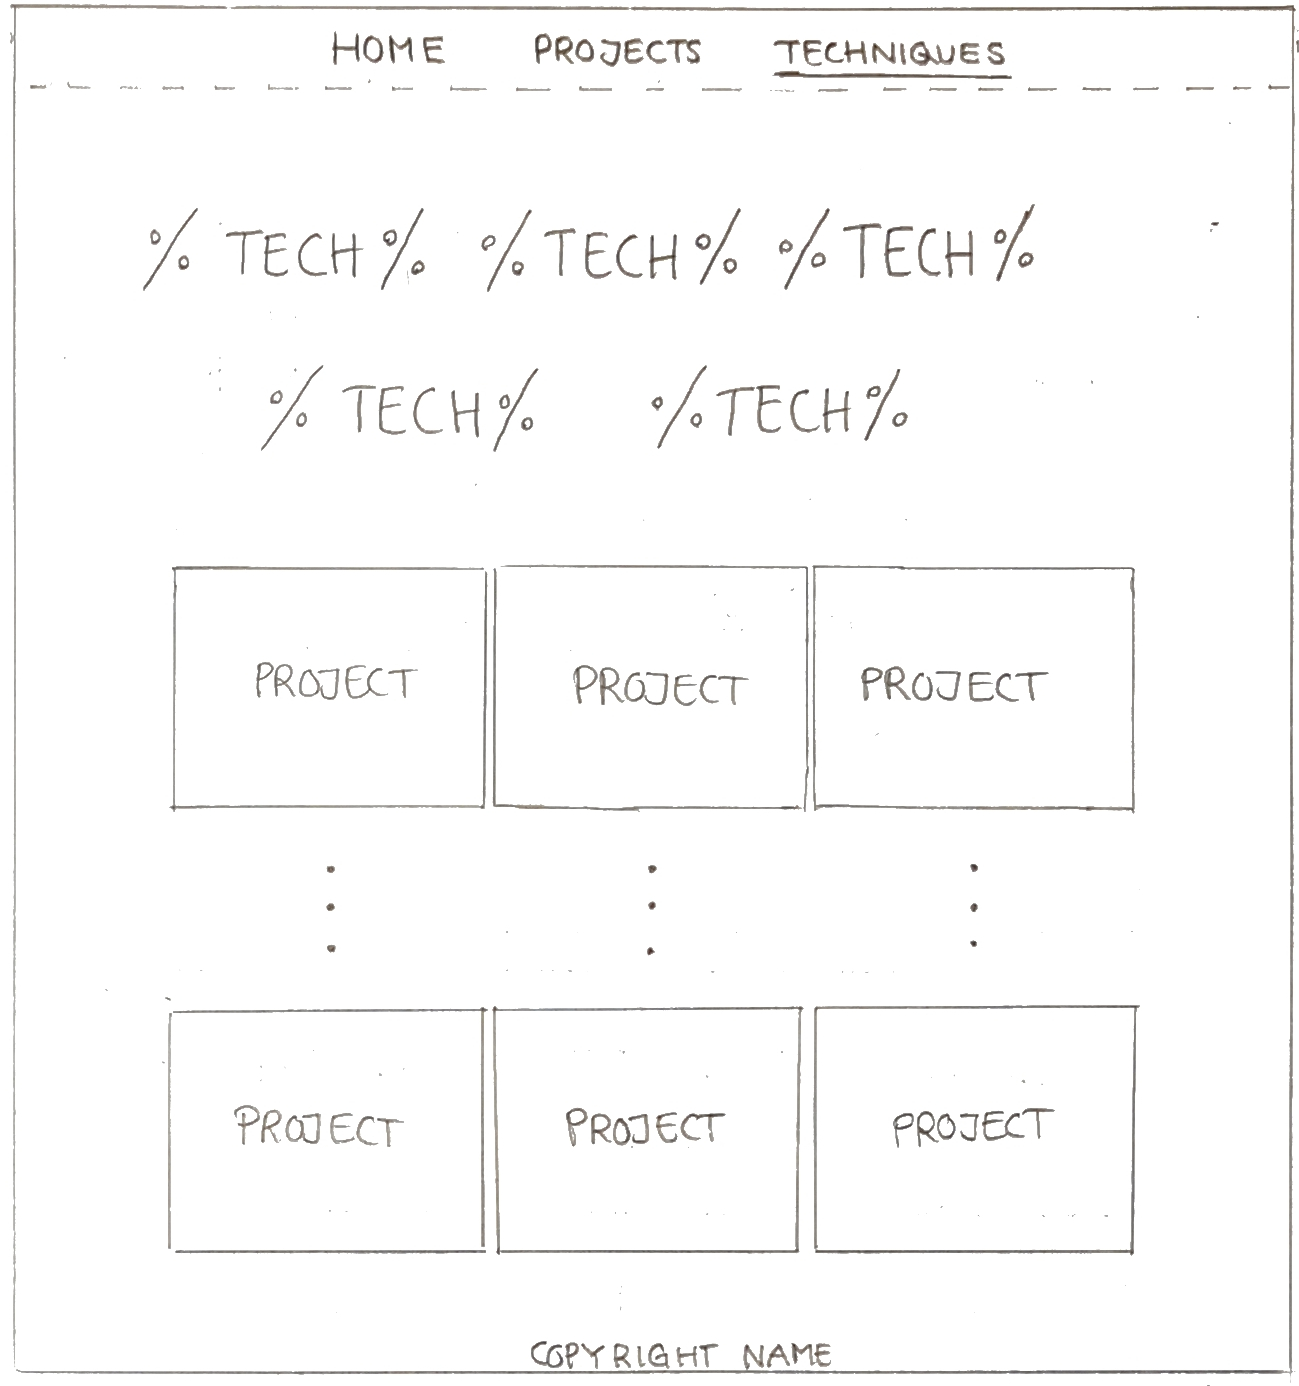
\includegraphics[width=120mm]{5_techniques.jpg}
  \caption{Tekniksidan} \label{fig4:Techniques}
\end{figure}

Tekniksidan ska visa alla tekniker som någon gång använts av utvecklaren.
En användare som navigerat till tekniksidan ska kunna trycka på en teknik för att sedan visa en lista med samtliga projekt som använder sig av den valda tekniken.

Det ska även vara möjligt att lägga till fler tekniker. Teknikerna ska visas upp till tre per rad och vara centrerade.
Ytterligare rader läggs till allteftersom fler tekniker läggs till. Sista raden kan därför innehålla endast en eller två tekniker.
\%TECH\%, se. Figur~\ref{fig4:Techniques} representerar en teknik. Varje teknik har en ikon som visar namnet på tekniken och möjligen en logotyp som är relevant för tekniken.

Projektlistan ska innehålla ett antal bilder som går att trycka på för att komma till det specifika projektets sida.
När användaren håller muspekaren över ett projekt så ska en kort beskrivning av projektet visas framför projektbilden.
Precis som med tekniker så kan sista raden i projektlistan innehålla mindre än tre projekt och sista raden kommer då centreras.

\pagebreak
\subsection{Enskilda projekt} \label{EnskildaProjekt}

\begin{figure}[ht!]
  \centering
  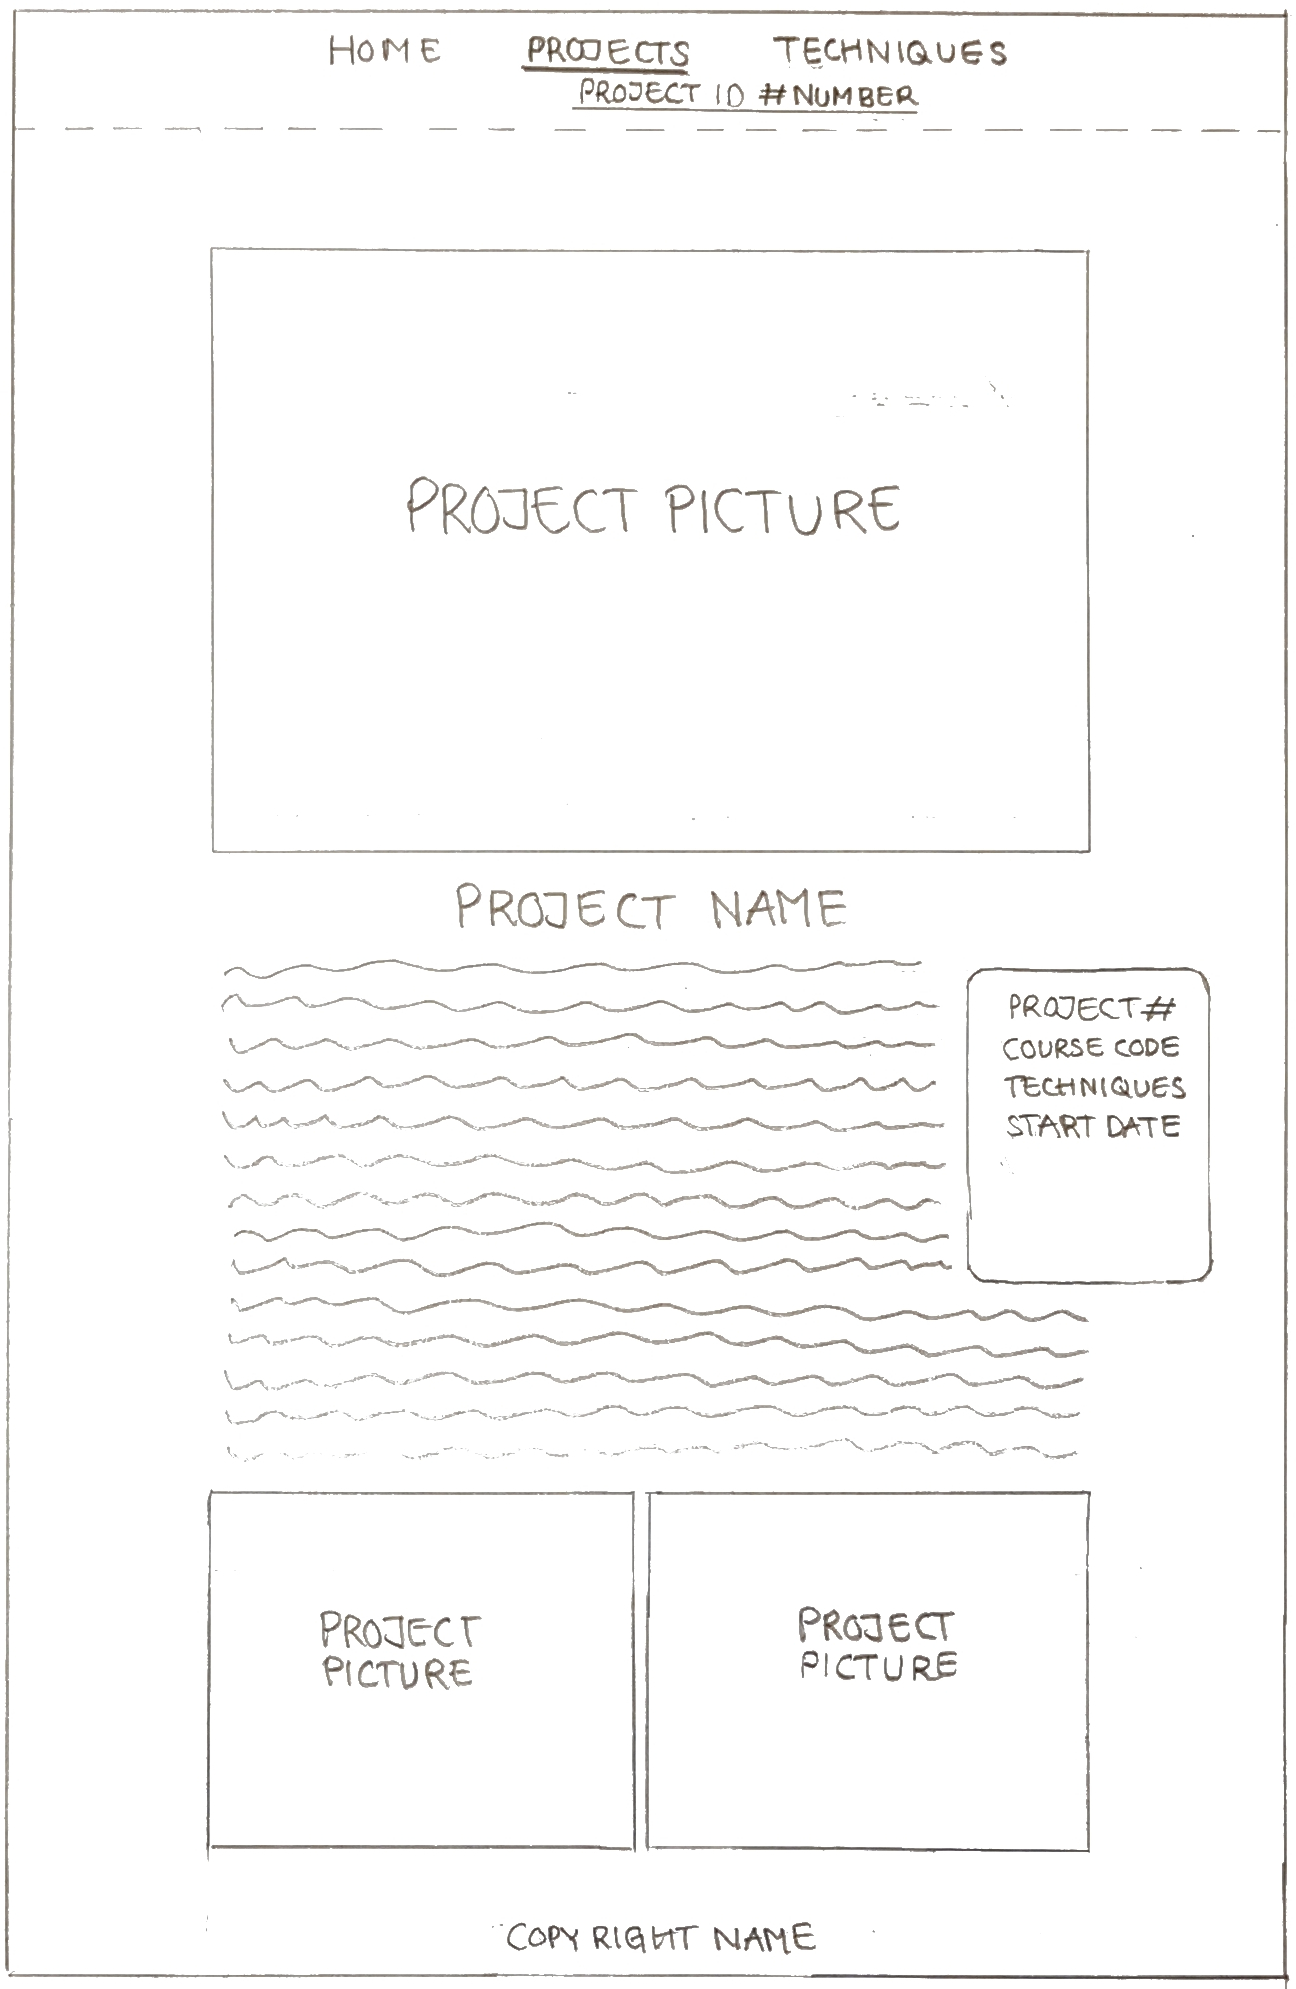
\includegraphics[width=110mm]{4_projectID.jpg}
  \caption{Sida för enkilt projekt.} \label{fig5:ProjectID}
\end{figure}

Det enskilda projektets sida, se Figur~\ref{fig5:ProjectID} presenteras med en stor bild på projektet i toppen av sidan.
Där kan man läsa mer om projektet och få information som t.ex. projektnamn, projekt-ID, kurskod, tekniker samt start- och slutdatum.
Längst ned på sidan efter projektets beskrivning kan man lägga till kompletterande bilder till projektet.

\end{document}
